% Options for packages loaded elsewhere
\PassOptionsToPackage{unicode}{hyperref}
\PassOptionsToPackage{hyphens}{url}
%
\documentclass[
  10pt,
]{article}
\usepackage{lmodern}
\usepackage{amssymb,amsmath}
\usepackage{ifxetex,ifluatex}
\ifnum 0\ifxetex 1\fi\ifluatex 1\fi=0 % if pdftex
  \usepackage[T1]{fontenc}
  \usepackage[utf8]{inputenc}
  \usepackage{textcomp} % provide euro and other symbols
\else % if luatex or xetex
  \usepackage{unicode-math}
  \defaultfontfeatures{Scale=MatchLowercase}
  \defaultfontfeatures[\rmfamily]{Ligatures=TeX,Scale=1}
\fi
% Use upquote if available, for straight quotes in verbatim environments
\IfFileExists{upquote.sty}{\usepackage{upquote}}{}
\IfFileExists{microtype.sty}{% use microtype if available
  \usepackage[]{microtype}
  \UseMicrotypeSet[protrusion]{basicmath} % disable protrusion for tt fonts
}{}
\makeatletter
\@ifundefined{KOMAClassName}{% if non-KOMA class
  \IfFileExists{parskip.sty}{%
    \usepackage{parskip}
  }{% else
    \setlength{\parindent}{0pt}
    \setlength{\parskip}{6pt plus 2pt minus 1pt}}
}{% if KOMA class
  \KOMAoptions{parskip=half}}
\makeatother
\usepackage{xcolor}
\IfFileExists{xurl.sty}{\usepackage{xurl}}{} % add URL line breaks if available
\IfFileExists{bookmark.sty}{\usepackage{bookmark}}{\usepackage{hyperref}}
\hypersetup{
  pdftitle={Report},
  pdfauthor={Davide Roznowicz},
  hidelinks,
  pdfcreator={LaTeX via pandoc}}
\urlstyle{same} % disable monospaced font for URLs
\usepackage[margin=1in]{geometry}
\usepackage{graphicx,grffile}
\makeatletter
\def\maxwidth{\ifdim\Gin@nat@width>\linewidth\linewidth\else\Gin@nat@width\fi}
\def\maxheight{\ifdim\Gin@nat@height>\textheight\textheight\else\Gin@nat@height\fi}
\makeatother
% Scale images if necessary, so that they will not overflow the page
% margins by default, and it is still possible to overwrite the defaults
% using explicit options in \includegraphics[width, height, ...]{}
\setkeys{Gin}{width=\maxwidth,height=\maxheight,keepaspectratio}
% Set default figure placement to htbp
\makeatletter
\def\fps@figure{htbp}
\makeatother
\setlength{\emergencystretch}{3em} % prevent overfull lines
\providecommand{\tightlist}{%
  \setlength{\itemsep}{0pt}\setlength{\parskip}{0pt}}
\setcounter{secnumdepth}{-\maxdimen} % remove section numbering

\title{Report}
\usepackage{etoolbox}
\makeatletter
\providecommand{\subtitle}[1]{% add subtitle to \maketitle
  \apptocmd{\@title}{\par {\large #1 \par}}{}{}
}
\makeatother
\subtitle{Assignment 1 - HPC}
\author{Davide Roznowicz}
\date{2/11/2020}

\begin{document}
\maketitle

{
\setcounter{tocdepth}{2}
\tableofcontents
}
\hypertarget{section-1-theoretical-model}{%
\section{Section 1: theoretical
model}\label{section-1-theoretical-model}}

\hypertarget{analysis-and-visual-comparisons-between-naive-and-enhanced-parallel-algorithms}{%
\subsection{Analysis and visual comparisons between naive and enhanced
parallel
algorithms}\label{analysis-and-visual-comparisons-between-naive-and-enhanced-parallel-algorithms}}

In order not to repeat similar plots a lot of times, I decided to insert
the enhanced version together with the naive one (in the same plot) from
the very beginning. However, the explanation concerning how the enhanced
algorithm was thought and built will be provided only after these visual
representations.

The first series of plots shows the total time the algorithms (serial,
naive and enhanced) need to perform the assigned task, varying the
number of cores P from 0 to 100 on the x-axis. N is fixed: the first
value given to to it is \(10^{4}\), then \(10^{5}\), \(10^{6}\),
\(10^{7}\). The time is calculated in the following way:
\[T_{serial}= T_{read} + N*T_{comp}\]
\[T_{naive}(P)= T_{comp}\times (P -1 + \frac{N}{P}) + T_{read} + 2(P-1)\times T_{comm}\]
\[T_{enhanced}(P)= 2\times T_{comm}\times \lceil{log_2(P)}\rceil)+T_{read}+(\frac{N}{P}+\lceil{log2(P)}\rceil)\times T_{comp}\]
Notice that, despite the fact that the exercise does not show
\(T_{read}\) in \(T_{serial}\) equation, I believe it should be taken
into consideration anyway: that's way it has been inserted into the
equation.

\begin{center}\rule{0.5\linewidth}{0.5pt}\end{center}

\begin{center}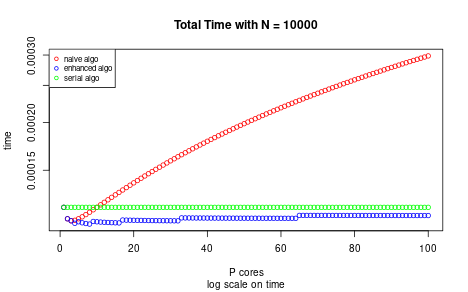
\includegraphics{figs/time_plots_naive_&_enhanced-1} \end{center}

\begin{center}\rule{0.5\linewidth}{0.5pt}\end{center}

\begin{center}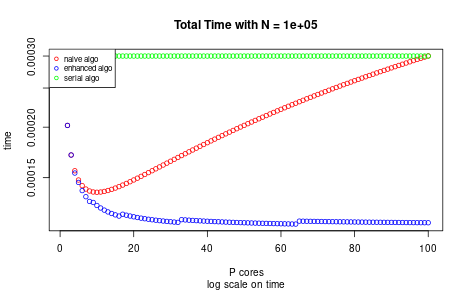
\includegraphics{figs/time_plots_naive_&_enhanced-2} \end{center}

\begin{center}\rule{0.5\linewidth}{0.5pt}\end{center}

\begin{center}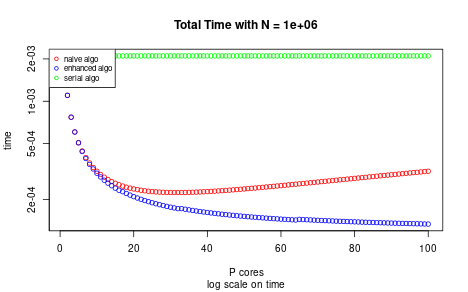
\includegraphics{figs/time_plots_naive_&_enhanced-3} \end{center}

\begin{center}\rule{0.5\linewidth}{0.5pt}\end{center}

\begin{center}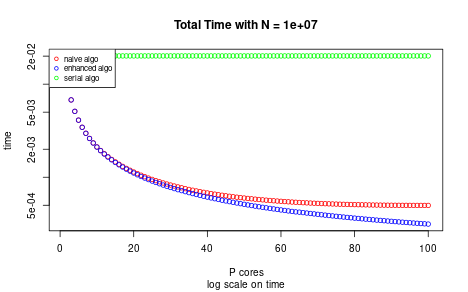
\includegraphics{figs/time_plots_naive_&_enhanced-4} \end{center}

The second series of plots shows the scalability of the algorithms
(serial, naive and enhanced), varying the number of cores P on the
x-axis. N is fixed again to the previously mentioned values.

\begin{center}\rule{0.5\linewidth}{0.5pt}\end{center}

\begin{center}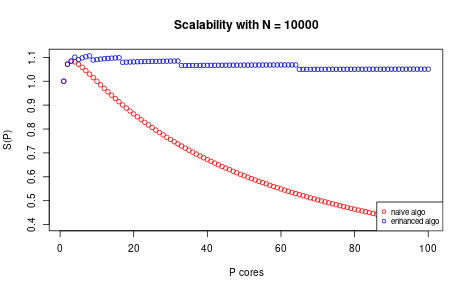
\includegraphics{figs/scalability_plots_naive_&_enhanced-1} \end{center}

\begin{center}\rule{0.5\linewidth}{0.5pt}\end{center}

\begin{center}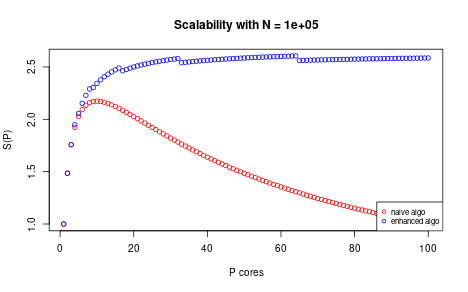
\includegraphics{figs/scalability_plots_naive_&_enhanced-2} \end{center}

\begin{center}\rule{0.5\linewidth}{0.5pt}\end{center}

\begin{center}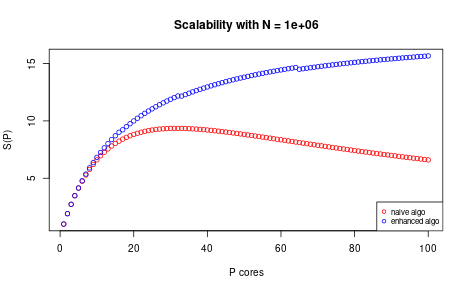
\includegraphics{figs/scalability_plots_naive_&_enhanced-3} \end{center}

\begin{center}\rule{0.5\linewidth}{0.5pt}\end{center}

\begin{center}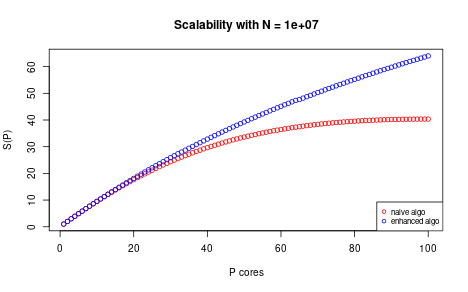
\includegraphics{figs/scalability_plots_naive_&_enhanced-4} \end{center}

\hypertarget{for-which-values-of-n-do-you-see-the-algorithm-scaling}{%
\subsection{For which values of N do you see the algorithm scaling
?}\label{for-which-values-of-n-do-you-see-the-algorithm-scaling}}

We easily notice that the higher N is, the better the parallel
algorithms scale. Except for N and P very small, case in which
\(T_{comm}\) represents a large and unnecessary overhead, the enhanced
algorithm tends to be far more scalable than the naive version.

\hypertarget{for-which-values-of-p-does-the-algorithm-produce-the-best-results}{%
\subsection{For which values of P does the algorithm produce the best
results
?}\label{for-which-values-of-p-does-the-algorithm-produce-the-best-results}}

Notice: the considered range for P is {[}1,100{]}, as stated in the
exercise requests.

\begin{verbatim}
## [1] "if N = 10000 , the best P for naive algo is : 3"
## [1] "if N = 10000 , the best P for enhanced algo is : 8"
## [1] "if N = 1e+05 , the best P for naive algo is : 10"
## [1] "if N = 1e+05 , the best P for enhanced algo is : 64"
## [1] "if N = 1e+06 , the best P for naive algo is : 32"
## [1] "if N = 1e+06 , the best P for enhanced algo is : 100"
## [1] "if N = 1e+07 , the best P for naive algo is : 100"
## [1] "if N = 1e+07 , the best P for enhanced algo is : 100"
\end{verbatim}

Therefore it is clear that if N grows, so does the best P both for naive
and enhanced algorithms. As pointed before, the communication time is a
huge overhead for the naive algorithm: in fact, unless N is very large
(and also \(\frac{N}{P}\) is large), its scalability curve tends to
flatten almost immediately and then go down. This happens because the
increasing number of cores cannot sustain easily the rapid growth of
\(T_{comm}\), that is by the way three orders of magnitude more
influential than \(T_{comp}\). Instead, if N is large enough, the
scalabily curve of the enhanced algorithm is much more ``resilient''
than the one belonging to the naive version, thus the best P tends to be
much higher: this is mainly associated with the improvements concerning
the designed communication system, such that it is not linearly
dependent on P, but instead logarithmically dependent.

\hypertarget{can-you-try-to-modify-the-algorithm-sketched-above-to-increase-its-scalability-hints-try-to-think-of-a-better-communication-algorithm}{%
\subsection{Can you try to modify the algorithm sketched above to
increase its scalability ? (hints: try to think of a better
communication
algorithm)}\label{can-you-try-to-modify-the-algorithm-sketched-above-to-increase-its-scalability-hints-try-to-think-of-a-better-communication-algorithm}}

The enhanced version of the naive algorithm is designed thinking that
there is no particular sense in compelling the master core to send all
the ``messagges'' sequentially. Instead it seems much more convenient to
let other cores ``help'' the master in spreading the assigned task.
Thus, the optimal choice appears to be the following:

\begin{enumerate}
\def\labelenumi{\arabic{enumi}.}
\tightlist
\item
  After reading the task, the \(master\) should send half of the numbers
  to \(core_1\) and keep the other half for itself;
\item
  the \(master\) and \(core_1\) send half of their remaining numbers to
  \(core_2\) and \(core_3\) respectively;
\item
  the \(master\), \(core_1\), \(core_2\), \(core_3\) send half of their
  remaining numbers to \(core_4\), \(core_5\), \(core_6\), \(core_7\)
  respectively;
\item
  \ldots{} so on up to reaching \(core_{P-1}\);
\item
  the sums are crunched by the P cores (each core has the same amount of
  numbers);
\item
  the computed P-1 sums are sent back to master following the route
  provided in the first four phases but in reverse order; at each step
  the partial sums are computed in the slave cores and then sent to
  another core as described before; this is repeated until only the
  \(master\) and \(core_1\) have the partial sums (\(master\) has the
  sum of half of the amount of the original N numbers, while \(core_1\)
  has the other half);
\item
  \(core_1\) gives to the \(master\) its partial sum and the \(master\)
  computes the final sum;
\end{enumerate}

This way many of the ``steps'' for fully spreading an equal amount of
numbers to each core are done in parallel and not just sequentially like
in the naive algorithm.

Therefore:

\begin{itemize}
\tightlist
\item
  \(\sum_{k=0}^{steps-1} 2^k \geq P-1\)
\item
  \(\frac{1-2^{steps}}{1-2} \geq P-1\)
\item
  \(2^{steps}-1 \geq P-1\)
\item
  \(2^{steps} \geq P\)
\item
  \(steps \geq \frac{\log(P)}{\log(2)}\)
\item
  \(steps \geq \log_2{P}\)
\end{itemize}

However, due to the discrete context, \(\lceil{\log_{2}{P}}\rceil\)
should be considered instead of \(\log_2{P}\). Thus, the minimum is
\(steps=\lceil{\log_{2}{P}}\rceil\).

\begin{itemize}
\tightlist
\item
  Read N and distribute N to P-1 slaves ===\textgreater{}
  \(T_{read}+\lceil{\log_{2}{P}}\rceil \times T_{comm}\)
\item
  \(\frac{N}{P}\) sum over each processors (including master)
  ===\textgreater{} \(T_{comp}\times\frac{N}{P}\)
\item
  Slaves send partial sum ===\textgreater{}
  \(\lceil{\log_{2}{P}}\rceil \times T_{comm}\)
\item
  Slaves perform partial sums while sending back the numbers to the
  \(master\) ===\textgreater{}
  \((\lceil{\log_{2}{P}}\rceil-1) \times T_{comp}\)
\item
  Master performs one final sum ===\textgreater{} \(T_{comp}\)
\end{itemize}

The final model:
\[T_{enhanced}(P)= 2\times T_{comm}\times \lceil{log_2(P)}\rceil)+T_{read}+(\frac{N}{P}+\lceil{log2(P)}\rceil)\times T_{comp}\]
This enhanced algorithm not only improves the communication time because
of a faster way to send the equal amount of numbers to each core (and
then in the reverse process of getting them back), but also manages to
crunch the partial sums at the slaves level, in order to process
everything in parallel as much as possible.

\hypertarget{performance-model.csv}{%
\subsection{performance-model.csv}\label{performance-model.csv}}

The considered range for P is {[}1,100{]}, as stated in the exercise
requests. In the .csv the following results have been written down:

\begin{verbatim}
## [1] "if N = 20000 , the best P for naive algo is : 4"
## [1] "if N = 20000 , the best P for enhanced algo is : 16"
## [1] "if N = 1e+05 , the best P for naive algo is : 10"
## [1] "if N = 1e+05 , the best P for enhanced algo is : 64"
## [1] "if N = 2e+05 , the best P for naive algo is : 14"
## [1] "if N = 2e+05 , the best P for enhanced algo is : 100"
## [1] "if N = 1e+06 , the best P for naive algo is : 32"
## [1] "if N = 1e+06 , the best P for enhanced algo is : 100"
## [1] "if N = 2e+07 , the best P for naive algo is : 100"
## [1] "if N = 2e+07 , the best P for enhanced algo is : 100"
\end{verbatim}

\hypertarget{section-2-play-with-mpi-program}{%
\section{Section 2 : play with MPI
program}\label{section-2-play-with-mpi-program}}

\hypertarget{compute-strong-scalability-of-a-mpi_pi.c-program}{%
\subsection{2.1: compute strong scalability of a mpi\_pi.c
program}\label{compute-strong-scalability-of-a-mpi_pi.c-program}}

\hypertarget{single-core-serial-versus-single-core-parallel}{%
\subsubsection{Single core serial versus single core
parallel}\label{single-core-serial-versus-single-core-parallel}}

The serial calculation of pi with \(10^8\) iterations takes
\textasciitilde2.620 seconds, both for internally measured walltime and
externally computed elapsed time (by /usr/bin/time). Instead the
parallel calculation of pi with \(10^8\) iterations takes
\textasciitilde2.575 as walltime that is quite close to the serial
version. However the total elapsed time is higher \textasciitilde2.830
seconds. This is because, despite the fact that there are no
communication times among the cores (there is a single core), we should
take into account the overhead associated with starting the parallel
version of the program (system calls, starting machinaries\ldots) :
system time is not negligible (\textasciitilde0.13 seconds) as it was
before in the serial context. Moreover, the elapsed time is larger than
the walltime also because it includes printing the outcome of the
simulation. Of course, as a consequence, \(\%CPU=\frac{user}{elapsed}\)
is lower in the parallel version.

\hypertarget{strong-scalability}{%
\subsubsection{Strong scalability}\label{strong-scalability}}

The walltime related to the master core will be used to fill in the .csv
and perform the requested analysis: in fact, as we are interested in the
highest time among the cores, the master seems to be a good choice.

Let's look at some plots comparing the walltime (average among the three
runs) and elapsed time against the number of cores. The serial walltime
is also added for further comparison.

\begin{center}\rule{0.5\linewidth}{0.5pt}\end{center}

\begin{center}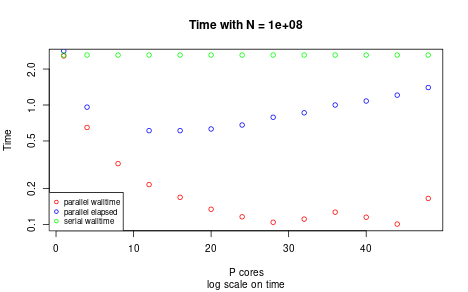
\includegraphics{figs/ss_time-1} \end{center}

\begin{center}\rule{0.5\linewidth}{0.5pt}\end{center}

\begin{center}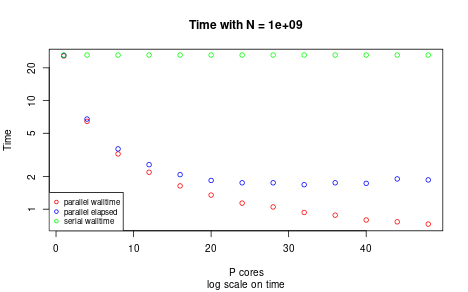
\includegraphics{figs/ss_time-2} \end{center}

\begin{center}\rule{0.5\linewidth}{0.5pt}\end{center}

\begin{center}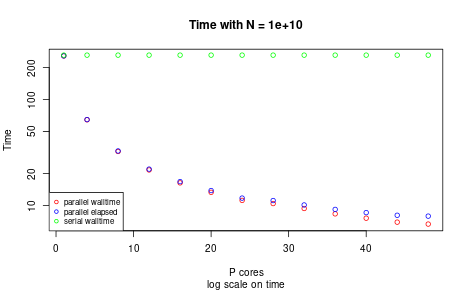
\includegraphics{figs/ss_time-3} \end{center}

\begin{center}\rule{0.5\linewidth}{0.5pt}\end{center}

\begin{center}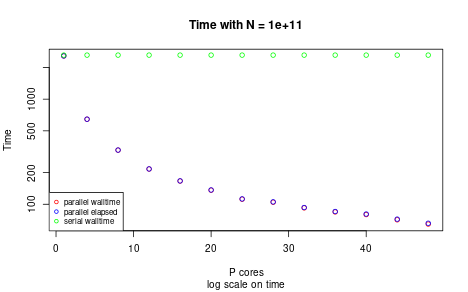
\includegraphics{figs/ss_time-4} \end{center}

As previously stated, the walltime dotted line for the parallel version
is always below the elapsed time, given the fact that it doesn't take
into consideration neither printing time nor additional system overhead.
The latter is particularly consistent when dealing with small sizes of
N; when N grows the relative weight of this factor for the simulation
time gets less visible. Notice that in the serial version, even though N
changes, the system time remains \textasciitilde0.00 while walltime and
elapsed time are almost the same.

Now let's look at scalability plots: 4 scalability curves for each size
of N are drawn in the same chart. As a matter of comparison, the
walltime is chosen to compute the scalability funcion: otherwise there
would be some components such as printing or system that might skew the
outcome as they also include some factors that are constant (but
difficult to see). Choosing the walltime allows us to focus on
scalability by spotting how communication times among cores (included in
walltime) affect the curves. As one-core-benchmark for computing
scalability we opt for the parallel version since the time is very close
to the serial one. Lines connecting the dots are drawn because points
would be too confusing for visualization.

\begin{center}\rule{0.5\linewidth}{0.5pt}\end{center}

\begin{center}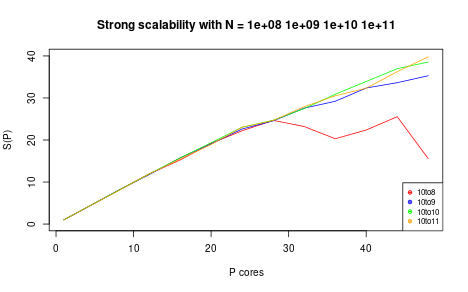
\includegraphics{figs/ss_scal-1} \end{center}

We easily notice that the higher N is, the better the parallel algorithm
scales and approximates a straight line. Up to 24 cores there's almost
perfect speed-up for all the involved sizes of N; later some
break-points appear according to the size of N. When N is small,
communication times heavily affect the outcome, thus the curves flatten.
Some swings are evident in the final parts of the curves: these are due
to some noise particularly evident when the time to perform the
simulation is in the order of a couple of seconds for one core
(e.g.~\(N=10^8\)).

\hypertarget{identify-a-model-for-the-parallel-overhead}{%
\subsection{2.2: identify a model for the parallel
overhead}\label{identify-a-model-for-the-parallel-overhead}}

Looking back at the time charts for strong scalability, it seems that
there is a linear dependence on P: in fact, after fixing N, we have that
as P grows so does the absolute difference among walltime and total
elapsed time. The main time components included in ``elapsed'' but not
in ``walltime'' are the system and the printing. Despite the fact there
might be constant terms, the number of printed sentences seems
increasing proportionally to the number of cores; similarly, the time
required to spawn and synchronize parallel tasks gives the impression to
be somehow expanding with P. Let's try to visualize the plots of this
absolute difference; then let's fit a regression model:

\begin{center}\rule{0.5\linewidth}{0.5pt}\end{center}

\begin{center}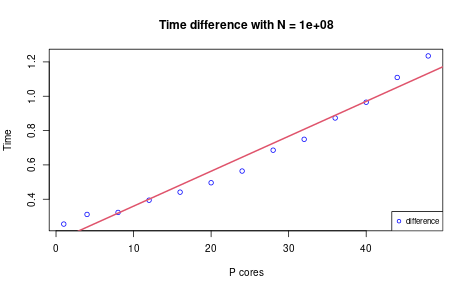
\includegraphics{figs/ws_overhead-1} \end{center}

\begin{verbatim}
## 
## Call:
## lm(formula = diffr ~ P_seq)
## 
## Residuals:
##       Min        1Q    Median        3Q       Max 
## -0.080643 -0.040750 -0.006134  0.057404  0.101460 
## 
## Coefficients:
##             Estimate Std. Error t value Pr(>|t|)    
## (Intercept) 0.156191   0.033160    4.71 0.000639 ***
## P_seq       0.020355   0.001172   17.36 2.42e-09 ***
## ---
## Signif. codes:  0 '***' 0.001 '**' 0.01 '*' 0.05 '.' 0.1 ' ' 1
## 
## Residual standard error: 0.06275 on 11 degrees of freedom
## Multiple R-squared:  0.9648, Adjusted R-squared:  0.9616 
## F-statistic: 301.5 on 1 and 11 DF,  p-value: 2.422e-09
\end{verbatim}

\begin{center}\rule{0.5\linewidth}{0.5pt}\end{center}

\begin{center}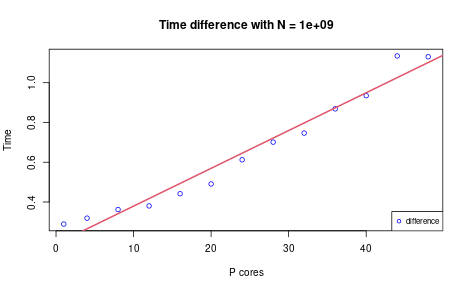
\includegraphics{figs/ws_overhead-2} \end{center}

\begin{verbatim}
## 
## Call:
## lm(formula = diffr2 ~ P_seq)
## 
## Residuals:
##      Min       1Q   Median       3Q      Max 
## -0.07873 -0.03712 -0.01500  0.02873  0.10904 
## 
## Coefficients:
##             Estimate Std. Error t value Pr(>|t|)    
## (Intercept) 0.189402   0.030705   6.168 7.02e-05 ***
## P_seq       0.019003   0.001086  17.505 2.22e-09 ***
## ---
## Signif. codes:  0 '***' 0.001 '**' 0.01 '*' 0.05 '.' 0.1 ' ' 1
## 
## Residual standard error: 0.0581 on 11 degrees of freedom
## Multiple R-squared:  0.9653, Adjusted R-squared:  0.9622 
## F-statistic: 306.4 on 1 and 11 DF,  p-value: 2.221e-09
\end{verbatim}

\begin{center}\rule{0.5\linewidth}{0.5pt}\end{center}

\begin{center}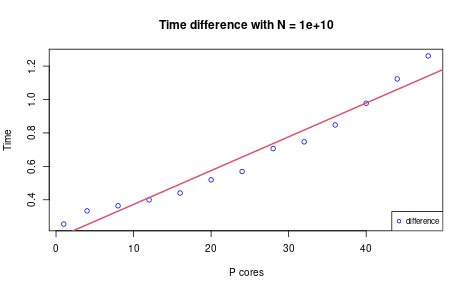
\includegraphics{figs/ws_overhead-3} \end{center}

\begin{verbatim}
## 
## Call:
## lm(formula = diffr3 ~ P_seq)
## 
## Residuals:
##      Min       1Q   Median       3Q      Max 
## -0.08644 -0.05338 -0.01337  0.06315  0.11994 
## 
## Coefficients:
##             Estimate Std. Error t value Pr(>|t|)    
## (Intercept) 0.170186   0.036450   4.669 0.000684 ***
## P_seq       0.020222   0.001289  15.693 7.08e-09 ***
## ---
## Signif. codes:  0 '***' 0.001 '**' 0.01 '*' 0.05 '.' 0.1 ' ' 1
## 
## Residual standard error: 0.06897 on 11 degrees of freedom
## Multiple R-squared:  0.9572, Adjusted R-squared:  0.9534 
## F-statistic: 246.3 on 1 and 11 DF,  p-value: 7.079e-09
\end{verbatim}

\begin{center}\rule{0.5\linewidth}{0.5pt}\end{center}

\begin{center}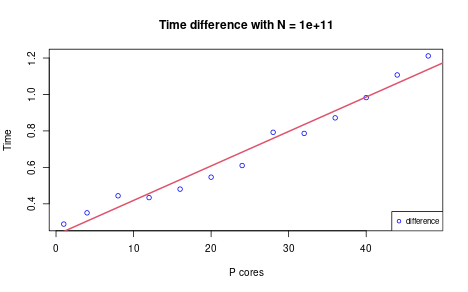
\includegraphics{figs/ws_overhead-4} \end{center}

\begin{verbatim}
## 
## Call:
## lm(formula = diffr4 ~ P_seq)
## 
## Residuals:
##       Min        1Q    Median        3Q       Max 
## -0.073559 -0.048548 -0.003333  0.045057  0.073909 
## 
## Coefficients:
##             Estimate Std. Error t value Pr(>|t|)    
## (Intercept) 0.229713   0.028725   7.997 6.56e-06 ***
## P_seq       0.018914   0.001016  18.624 1.15e-09 ***
## ---
## Signif. codes:  0 '***' 0.001 '**' 0.01 '*' 0.05 '.' 0.1 ' ' 1
## 
## Residual standard error: 0.05436 on 11 degrees of freedom
## Multiple R-squared:  0.9693, Adjusted R-squared:  0.9665 
## F-statistic: 346.9 on 1 and 11 DF,  p-value: 1.146e-09
\end{verbatim}

At first glance it would look like a regression line works perfectly.
This is confirmed by the stats of the regression showing very similar
slope coefficients (values between 0.018804 and 0.020355) for each
computed regression: therefore it seems N doesn't have meaningful impact
in the overhead function. Moreover we discover that the p-values
associated with the slope coefficients are very small (order of
\(10^{-9}\)): thus we reject the hypothesis of coeff\(=0\). Also the
intercept coefficients are not far from each other (between 0.156191 and
0.234349). We can conclude that there is a strong relationship of linear
dependence on P and precisely: \[T_{overhead}(P)\approx c + k\times P\]
where the intercept \(c\) is likely to be in the 95\% confidence
interval 0.1863731 \(\pm\) 0.03194011; while the slope coefficient \(k\)
should be included in 0.01962321 \(\pm\) 0.0007708309.

\hypertarget{weak-scaling}{%
\subsection{2.3: weak scaling}\label{weak-scaling}}

Let's look at the plots for weak scalability.

\begin{center}\rule{0.5\linewidth}{0.5pt}\end{center}

\begin{center}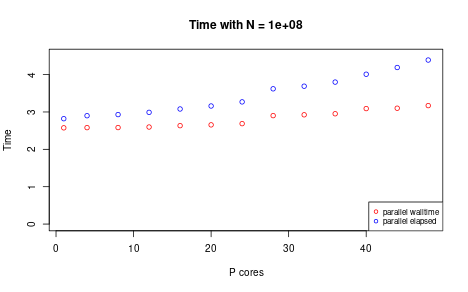
\includegraphics{figs/ws_time-1} \end{center}

\begin{center}\rule{0.5\linewidth}{0.5pt}\end{center}

\begin{center}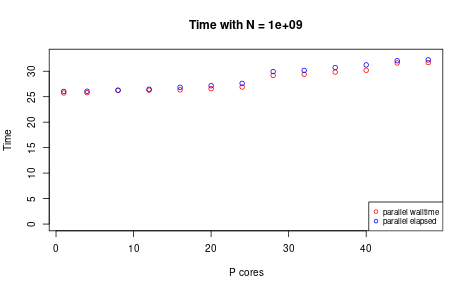
\includegraphics{figs/ws_time-2} \end{center}

\begin{center}\rule{0.5\linewidth}{0.5pt}\end{center}

\begin{center}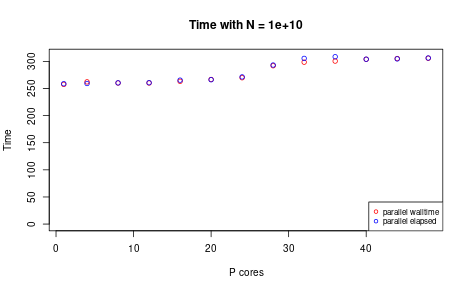
\includegraphics{figs/ws_time-3} \end{center}

\begin{center}\rule{0.5\linewidth}{0.5pt}\end{center}

\begin{center}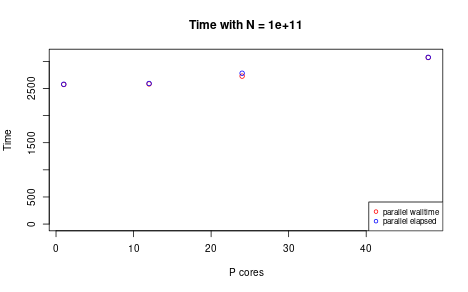
\includegraphics{figs/ws_time-4} \end{center}

According to perfect weak scalability, time should remain constant;
actually in the plots we see that there are no perfect horizontal lines:
that's because walltime includes communication time among the cores
lifting the overall time as P increases (logarithmically according to
the enhanced model described in the first section).

Let's look at the plots for weak scalability (weak efficiency function)
using walltime as before.

\begin{center}\rule{0.5\linewidth}{0.5pt}\end{center}

\begin{center}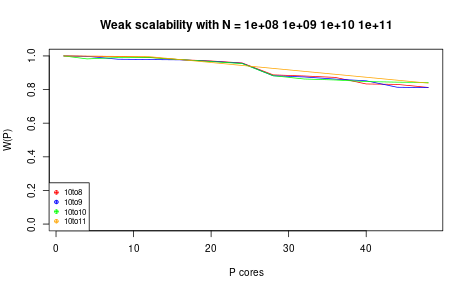
\includegraphics{figs/ws_scal-1} \end{center}

Again, theoretically speaking \(\frac{T(1)}{T(P)}\) should stay
constant. However as expected, we see curves slightly skewed towards the
bottom of the chart. The line referred to weak efficiency for
\(N=10^{11}\) is not so accurate because of the very few data points
available. Despite this fact, the curves tend to share a very similar
and close path: it is probably due to the fact that we were required to
increse the number of iterations linearly with the number of cores, thus
approaching the straight line limit (here it would be a horizonatal
line) as in strong scalability (when the number N was big).

\end{document}
